\chapter{Niveau 1}
\begin{figure*}[b]
  \centering
  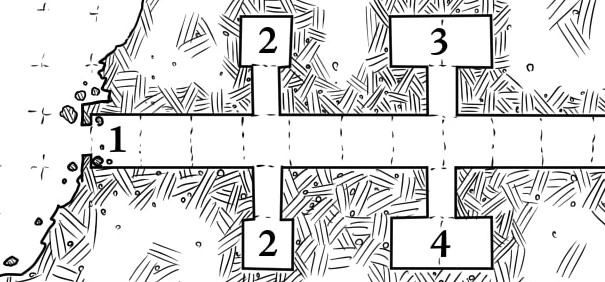
\includegraphics[width=0.7\linewidth]{pics/map_1-4.jpg}
\end{figure*}
\subsection{1 : Hall d’Entrée}\label{n1:s1}
\begin{itemize}
  \item Couloir de 18m de long, sur 1.5m de large.
  \item 2 ouvertures de 1m de large chaque côté. 
  \item Se termine par une porte barrée menant en \textbf{\nameref{n1:s6}}.
\end{itemize}

\subsection{2 : Tombes des Gardes}\label{n1:s2}
Ces petites salles sont identiques en termes de taille et contenu. 
Chacune contient un cercueil de bois renfermant une statue d'homme-serpent en argile.

\begin{itemize}
  \item Statue de \emph{guerrier} creuse, contient :
  \begin{itemize}
    \item une amulette d’or (10 PO)
    \item un squelette de serpent desséché
  \end{itemize}
  \item Piège : nuage de gaz empoisonné (Sauvegarde Poison ou 1d6 dégâts)
\end{itemize}

%\begin{highlight}
%\textbf{Leçons : }le donjon est organisé, il contient des motifs.
%
%Il y a des trésors cachés, ainsi que des dangers cachés.
%Les PJ aborderont probablement le second cercueil avec bien plus de précautions que le premier, et pourront récupérer la récompense (or) tout en évitant le danger (poison) s’ils mettent à profit leur cerveau (et un caillou ou long bâton).
%\end{highlight}
\vfill\break
\subsection{3 : Tombe d’Érudit}\label{n1:s3}
Même chose que \textbf{\nameref{n1:s2}} aux différences :
\begin{itemize}
  \item Statue d'\emph{érudit} creuse
  \item Parchemins tombés en poussière
\end{itemize}

\subsection{4 : Tombe de Sorcier}\label{n1:s4}
Même chose que \textbf{\nameref{n1:s2}} aux différences :
\begin{itemize}
  \item Statue de \emph{sorcier} creuse
  \item Porte un anneau d’argent. Si arraché :
  \begin{itemize}
    \item Brise la statue
    \item Projette le poison
  \end{itemize}
\end{itemize}

\begin{highlight}[Anneau d’argent]
  \begin{itemize}
    \item magique \textbf{et} maudit
    \item Porté au doigt, l’ongle s’allonge et bifurque en deux pointes aiguisées comme des crocs.
    \item Mêmes effet qu'une dague empoisonnée : 
    \item Chaque matin  : Sauvegarde contre le poison ou 1d6 dégâts.
    \item Si 6 dégâts :  le doigt tombe et se transforme en serpent.
  \end{itemize}
\end{highlight}

%\begin{highlight}
%\textbf{Leçons :} Les trésors cachés peuvent être magiques, utiles et parfois maudits.
%\end{highlight}

\newpage
\begin{center}
  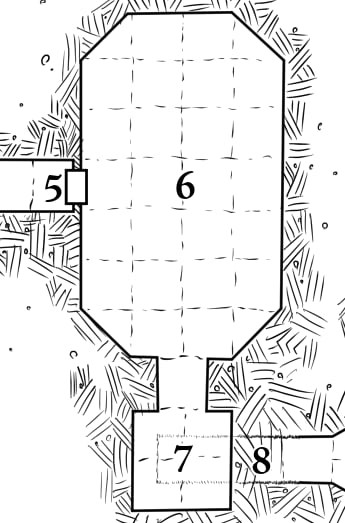
\includegraphics[width=\columnwidth]{pics/map_5-8.jpg}
\end{center} 

\subsection{5 : Porte / Marteau}\label{n1:s5}
Le corridor se termine par une porte barrée. 
Deux pieux de fer plantés de chaque côté du chambranle soutiennent une lourde barre de pierre, bloquant l’accès à la salle suivante.

\begin{itemize}
  \item 3 PJ au moins pour la soulever
  \item Soulevée : Piège (Sauvegarde Mort ou 2d6+4 dégâts).
\end{itemize}

\begin{highlight}[Le piège]
  \begin{itemize}
    \item Marteau de pierre bascule du plafond
    \item Remplit \emph{presque} intégralement le couloir
    \item \'Eviter :
    \begin{itemize}
      \item Se plaquer au mur
      \item S'aider d'un autre PJ pour prendre appui : +2 au jet, -2 à l'autre PJ.
    \end{itemize}
    \item Détection :
    \begin{itemize}
      \item Examiner la porte, le plafond
      \item Examiner les pieux : se redressent lentement lorsque la barre est soulevée
    \end{itemize}
    \item Désactiver :
    \begin{itemize}
      \item Replacer la barre
      \item Maintenir les pieux en position basse
      \item Endommager le mécanisme au plafond
    \end{itemize}
  \end{itemize}
\end{highlight}

%\begin{highlight}
%\textbf{Leçon :} certains pièges sont mortels. 
%Le donjon peut s’avérer létal.
%\end{highlight}

À moins que quelque chose ne le bloque, le marteau se rétracte lentement dans le plafond.
 
Il peut être activé à nouveau en abaissant les pieux de fer, à la main ou avec une corde. 

L’impact force violemment l’ouverture des portes menant en \textbf{\nameref{n1:s6}}


\subsection{6 : Fausse Tombe Royale}\label{n1:s6}
La chambre funéraire du roi des hommes-serpents et ses deux épouses. 
\begin{itemize}
  \item 3 cercueils de bois long du mur nord 
  \item Celui du milieu plus volumineux et ornementé.
  \item Contiennent chacun un squelette
  \item Attaquent dès que leur repos est troublé
\end{itemize}

\begin{table}[hb]
  \caption*{Squelette}
  \begin{osetable}{X[2]X[1]X[1]X[2]}{0}
    CA          & 7      & DV & 1 (4 pv) \\
    TACO        & 19 [0] & XP & 10 \\
    Attaque     & \SetCell[c=3]{l} 1D6 (griffes) & &\\
    Sauvegardes & \SetCell[c=3]{l} {\small MP~12 B~13 PP~14 S~15 SSB~16}& &\\
    Déplacement & 18m    & Moral & 12 \\
\end{osetable}
\end{table}

%\begin{highlight}
%\textbf{Leçons :} il y a des morts-vivants dans le donjon. 
%Ils sont moins sensibles aux armes tranchantes. 
%Il est possible d’utiliser l’environnement contre eux (en les attirant dans le piège à marteau).
%\end{highlight}

\subsection{7 : Faux Temple}\label{n1:s7}
\begin{itemize}
  \item Pièce dominée par une statue d’un dieu homme-serpent. 
  \begin{itemize}
    \item Gigantesque, Hideux
  \end{itemize}
  \item Eau suinte du plafond
  \item L'eau a érodé le sol
  \item Révèle \textbf{\nameref{n2:s8}} sous la sculpture vers le \textbf{\nameref{n2}} du donjon
\end{itemize}

%\begin{highlight}
%\textbf{Leçons :} il y a des passages secrets. 
%Ils sont associés aux statues. 
%Il pourrait s’agir d’une fausse tombe.
%Tout au long de ce donjon, les statues sont synonymes de passages secrets et de trésors.
%\end{highlight}